\chapter{Discussão dos Resultados}\label{cap_5_Resultados}

Neste capitulo será discutido os desafios, e soluções que levaram ao funcionamento do projeto de acordo com as especificações.

\section{O Circuito Completo}

\subsection{Desafios}

O maior desafio encontrado foi o entendimento de processos paralelos. 

Em geral, tinha-se uma tendencia a imaginar que bugs ou inconsistências lógicas do circuito ocorriam pois certas operações estavam fora de ordem.

Para fazer o debug dessa hipótese foi criado uma função buffer de 1bit, para ter-se melhor controle sobre a ordem das operações lógicas na placa. Ela pode ser vista na Figura \ref{fig:5.1}.

\begin{figure}[H]
	\centering
	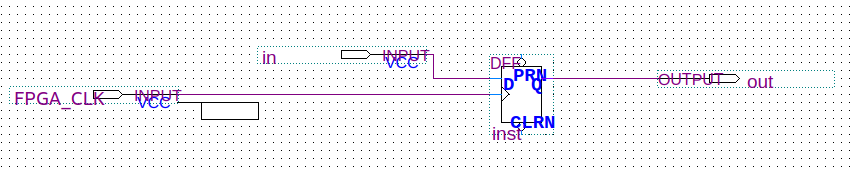
\includegraphics[width=1\columnwidth]{FIGURAS/cap_5/buffer_1bit.png}
	\caption{Buffer de 1 bit, que foi utilizado para debug.}
        \label{fig:5.1}
\end{figure}

Foi notado que em todos os casos que foi pensado que o bug ocorria por falta de paralelismo, o problema foi erros lógicos da parte do grupo.

Fazer descrição de hardware parece fundamentalmente diferente do que já havia-se visto antes, que foi programação imperativa e sequencial.

\subsection{Soluções}

%Não entendi essa segunda frase
A solução foi uma mudanca da maneira de pensar sobre descrição lógica. Isso para tentar realmente aceitar que os processos de fato ocorrem simultaneamente, e tentar manter lógicas sequenciais restritas a serem atreladas ao clock do FPGA.

\section{Flip-Flops}

\subsection{Desafios}

Não tinha-se costume com a ideia de clear e preset, apresentadas nas Figuras \ref{fig:2.2} e \ref{fig:2.3}.

Houve problemas com como causar um clear ou um preset em um devido flip-flop, sem o "travar" num valor de clear ou preset.

\subsection{Soluções}

Para resolver este problema, foi criado a função pulso, descrita na seção 2.6

Com esta, foi possível transformar um rising\_edge ou falling\_edge do clock como um pulso, que rapidamente ativa o clear ou o preset, e o desliga. Isso foi feito para causar um reset no flip-flop, mas mantê-lo em operação.

\section{Divisores}

\subsection{Desafios}

Foi criado um divisor simples, descrito na figura \ref{fig:2.4}, com lógica decrescente. Isso, devido aos requerimentos do projeto.

Ele funcionou de maneira bem direta. Porém, teve-se problema quando foi tentado o utilizar como contador crescente em cascata com outros Divisor1. Isso foi visto na seção 2.3.2.

O problema é que na primeira subida logica no modo crescente, o $Q$ subiria de 0 para 1. E se esse estiver no input clock do flip-flop seguinte, o seguinte também seria acionado e o $Q$ do seguinte subiria o nivel lógico.

Isso causa um efeito em cascata, no qual a primeira subida do clock inicial do primeiro flip-flop da cascata, acarreta que todos flip-flops são ativados e todos niveis lógicos de todos sobem.

Esse comportamento era indesejado.

\subsection{Soluções}

Com o \emph{Not} na saida do Divisor1, este problema foi resolvido. Isso ocorre já que na primeira subida logica do clock, haverá uma descida lógica da saída, o que não causa ativação do flip-flop seguinte.

\section{Contadores}

\subsection{Desafios}

A dificuldade central com contadores foi fazer o controle do reset e o controle de como o fazer ser crescente ou decrescente.

\subsection{Solucao}

No contador de 8 bits autoral, foi criado uma lógica crescente no contador. Esse contador pode ser feito crescente ou decrescente alterando apenas as suas saídas com um \emph{NOT}.

E com isso foi controlado, não o ponto de parada do contador, mas sim seu \emph{Modulo}. Ou seja. foi possível escolher se começa-se em $255$ ou $0$, e o reset ocorreria quando seu \emph{MOD} for atingido.


\section{Frequências acima de 1Hz}

\subsection{Desafios}

Poderia-se ter utilizado o LPM Counter para fazer a divisão, mas foi resolvido utilizar o contador autoral e divisor de frequência para fins didáticos.

O maior desafio foi definir a precisão que queria-se nas frequências.

\subsection{Soluções}

Pode-se fazer este ser mais preciso utilizando um contador de mais de 8 bits, ou múltiplos contadores de 8 bits.

Por fim resolveu-se escolher o valor que utilize o mínimo de componentes e tenha margem de erro de menos de $1\%$.

Isso permitiu utilizar apenas divisores simples e um contador 8 bits para obter cada frequência.

\section{Pulsos}

\subsection{Desafios}

Ele foi criado para resolver dois problemas. O primeiro foi que precisava-se que componentes fossem ativados tanto na subida de um clock, quanto na descida. O segundo foi o problema do rápido reset/preset de flip-flops.

\subsection{Soluções}

Este pulso resolveu ambos requerimentos e foi utilizado extensivamente no projeto.

\section{Debounce}

\subsection{Desafios}

Teve-se problemas ligando flip-flops diretamente nos push-buttons. 

Crê-se que isso ocorreu pelo botão ser um sistema mecânico e há uma transição imperfeita entre seu estado desligado para seu estado ligado. Isso acarretou que naquela transição, o nível lógico enviado pelo input sobe e desce uma quantidade não previsível de vezes.

\subsection{Soluções}

Foi implementado um debouncer para os botões, Figura \ref{fig:2.14}. Talvez ele funcionaria se utilizasse menos buffers e uma frequência mais alta, Porém, após ele funcionar, não foi tentado otimizá-lo mais.


\section{Registradores}

\subsection{Desafios}

Precisa-se de um sistema que armazene 16 hexadecimais, e faça o ciclo entre eles baseado em um \emph{Rising\_Edge} de entrada.

\subsection{Soluções}

Cria-se o registrador como sugerido, e com este, utiliza-se um contador MOD 16 para controlar a saída de um banco de registradores, alterando o qual registrador será a saída deste banco de registradores, baseado na contagem do contador.

E também usa-se o estouro \emph{Carry\_Out} do contador como o aviso para o sistema que todos hexadecimais foram inseridos corretamente.


\section{Prioridade}

\subsection{Desafios}

Foi encontrado um problema ao apertar um botão enquanto o buzzer estava reproduzindo uma frequência, isso fazia com que houvesse um conflito entre as frequências que foram enviadas ao buzzer. 

\subsection{Soluções}

Para resolver esse problema foi implementado um sistema de prioridades, visto na seção 2.9, que envia para o buzzer a frequência mais recente. Com isso, ao ser enviada alguma frequência, ela irá cancelar todas as outras frequências para enviar a mais recente para o buzzer.

\section{Comparador}

\subsection{Desafios}

Precisa-se de um sistema que realize a comparação entre a entrada do usuário e a senha armazenada nos registradores.

\subsection{Soluções}

Para ser feita a comparação, foi feito um sistema utilizando quatro portas lógicas XOR e uma NOR. Caso os bits nas entradas das portas lógicas XOR forem iguais, a saída delas será 0, portanto, se todas as entradas da porta lógica NOR forem 0 a saída será 1.

\section{LED e Buzzers}

\subsection{Desafios}

Teve-se problemas para conseguir que o buzzer desligue após certo tempo pré-determinado ligado.

\subsection{Soluções}

Utiliza-se o nível lógico do LED para ativar um flip-flop que ativa/desativa um mute switch do buzzer.

E utilizamos também o nível lógico deste mesmo flip-flop para iniciar um divisor de frequências de $2$ Hz que é inserido num contador decrescente MOD 2, como foi requisitado no projeto, isto nos dá uma frequência de saída de $1$ Hz, nesta frequência enviamos um pulso para o reset do flip-flop, para dar mute no buzzer.

\section{Display de sete segmentos}

\subsection{Desafios}

Ao realizar todas as funcionalidades obrigatórias, optamos por desenvolver uma funcionalidade extra ao projeto, que consiste na exibição da saída do contador MOD 10 decrescente no display de sete segmentos.

\subsection{Soluções}

Para isso, ao invés de utilizar apenas o clock de saída do contador MOD 10, monitoramos tambêm as saídas de seus flip-flops com o intuito de exibir em tempo real sua contagem no display de sete segmentos.